\documentclass[tikz,border=8pt]{standalone}
% Shared look for every TikZ diagram. Load with \input{../../tools/tikz-style.tex}
\usepackage[T1]{fontenc}
\usepackage{lmodern}
\renewcommand{\sfdefault}{lmr}  % diagrams use the same serif as the text
\usetikzlibrary{arrows.meta, positioning, shapes.geometric, calc, fit, backgrounds}
\definecolor{cblue}{HTML}{4C78A8}
\definecolor{corange}{HTML}{F58518}
\definecolor{cgreen}{HTML}{54A24B}
\definecolor{cred}{HTML}{E45756}
\definecolor{cpurple}{HTML}{B279A2}
\definecolor{cgrey}{HTML}{6B6B6B}
\tikzset{
  every picture/.style={font=\sffamily, line width=1.2pt},
  box/.style={draw=#1, fill=#1!12, rounded corners=4pt, align=center, inner sep=7pt, minimum height=1.1cm},
  box/.default=cgrey,
  arrow/.style={-{Stealth[length=3mm]}, draw=cgrey, line width=1.4pt},
  title/.style={font=\sffamily\bfseries\Large},
  note/.style={font=\sffamily\small, text=cgrey, align=center},
}
\AtBeginDocument{\hyphenpenalty=10000 \exhyphenpenalty=10000}

\begin{document}
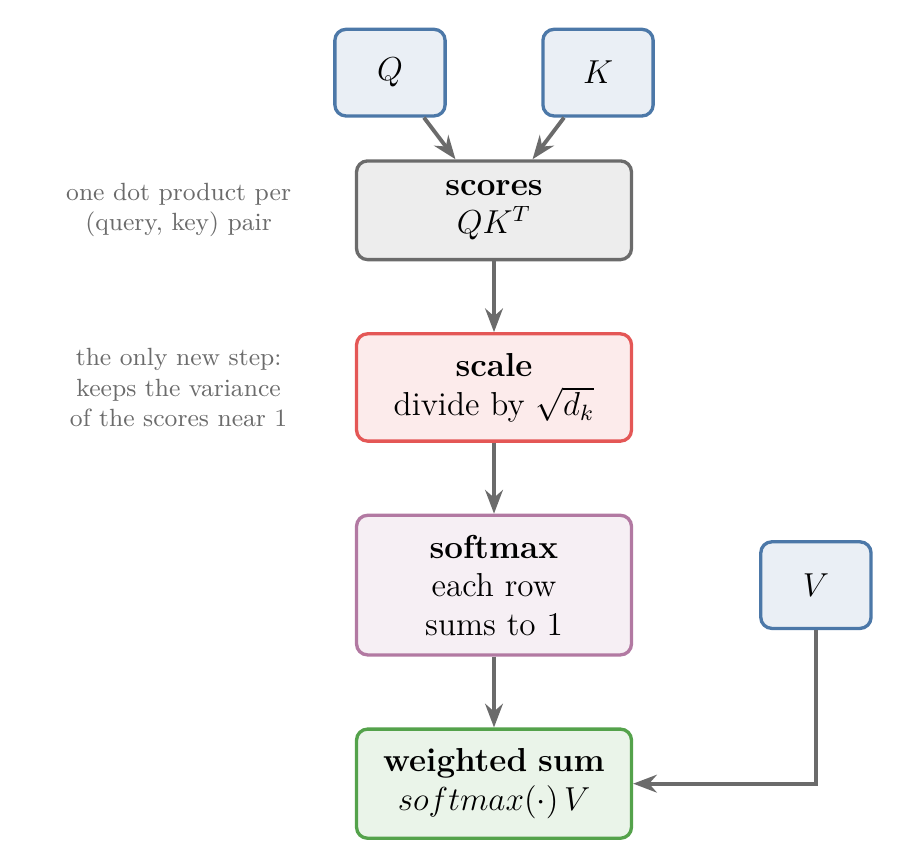
\begin{tikzpicture}[node distance=0.9cm, every node/.append style={font=\sffamily\large}]
  \node[box=cblue, minimum width=1.4cm] (q) {$Q$};
  \node[box=cblue, minimum width=1.4cm, right=1.2cm of q] (k) {$K$};
  \node[box=cgrey, text width=3.0cm, below=1.1cm of $(q)!0.5!(k)$] (mm) {\textbf{scores}\\$QK^{T}$};
  \node[box=cred, text width=3.0cm, below=of mm] (sc) {\textbf{scale}\\divide by $\sqrt{d_k}$};
  \node[box=cpurple, text width=3.0cm, below=of sc] (sm) {\textbf{softmax}\\each row sums to 1};
  \node[box=cblue, minimum width=1.4cm, right=1.6cm of sm] (v) {$V$};
  \node[box=cgreen, text width=3.0cm, below=of sm] (out) {\textbf{weighted sum}\\$\text{softmax}(\cdot)\,V$};
  \draw[arrow] (q) -- (mm); \draw[arrow] (k) -- (mm);
  \draw[arrow] (mm) -- (sc); \draw[arrow] (sc) -- (sm); \draw[arrow] (sm) -- (out);
  \draw[arrow] (v) |- (out);
  \node[note, left=0.3cm of sc, text width=3.6cm] {the only new step:\\keeps the variance\\of the scores near 1};
  \node[note, left=0.3cm of mm, text width=3.6cm] {one dot product per\\(query, key) pair};
\end{tikzpicture}
\end{document}
